\documentclass[10pt]{beamer}

%\usepackage[backend=bibtex,firstinits=true,style=verbose-inote,citestyle=authortitle]{biblatex}
\usepackage{bm}
\usepackage{graphicx}
\usepackage{subcaption}
\usepackage{amsmath}
\usepackage{amsfonts}
\usepackage{makecell}
\usepackage{filecontents}
\usepackage{biblatex}
\newcommand{\expect}[2][]{
\ifthenelse{\equal{#1}{}}{
\mathbb{E}\left[#2\right]
}{
\underset{#1}{\mathbb{E}}\left[#2\right]
}}

\newcommand{\cov}[2][]{
\ifthenelse{\equal{#1}{}}{
\text{Cov}\left[#2\right]
}{
\underset{#1}{\text{Cov}}\left[#2\right]
}}


\newcommand{\var}[2][]{
\ifthenelse{\equal{#1}{}}{
\text{Var}[#2]
}{
\underset{#1}{\text{Var}}[#2]
}}

\newcommand{\loss}[2][]{
\ifthenelse{\equal{#1}{}}{
\mathcal{L}(#2)
}{
\mathcal{L}_{#1}(#2)
}}

\newcommand{\kl}[2]{
\text{D}_\text{KL}[#1 \parallel #2]
}

\newcommand{\R}{\mathbb{R}}
%\newcommand{\Prob}{\mathbb{P}}

\newcommand{\1}[1]{\mathds{1}\{#1\}}


%\usecolortheme{dolphin}
\setbeamertemplate{navigation symbols}{}
\setbeamertemplate{section in toc}{\inserttocsectionnumber.~\inserttocsection}

\begin{filecontents*}{references.bib}
@inproceedings{BigGAN,
title={Large Scale {GAN} Training for High Fidelity Natural Image Synthesis},
author={Andrew Brock and Jeff Donahue and Karen Simonyan},
booktitle={International Conference on Learning Representations},
year={2019},
url={https://openreview.net/forum?id=B1xsqj09Fm},
}
\end{filecontents*}
\addbibresource{references.bib}


\title{Large Scale GAN Training for High Fidelity Natural Image Synthesis \footnote{\citepaper{BigGAN}}}
%\subtitle{}
%\author{Ivan Skorokhodov}
%\date{}
%\logo{
\includegraphics[height=1cm]{images/ipavlov-logo.png}}

\newcommand{\citepaper}[1]{\citetitle{#1} by \citeauthor{#1}}

%\graphicspath{{./images}}

%\usetheme{lucid}
\begin{document}

\begin{frame}
    \titlepage
\end{frame}

\begin{frame}{Main ideas}
    \pause
    \begin{itemize}
        \item\pause Authors trained the largest GAN model (to the moment of the project)
        \item\pause Explored a lot of techniques of training GANs
        \item\pause Proposed a ``truncation trick'' for better sampling at test-time
        \item\pause Dramatically improved SotA on ImageNet
    \end{itemize}
\end{frame}

\begin{frame}{Inception Score (IS)}
    \begin{enumerate}
        \item\pause Take Inception classifier
        \item\pause Generate a lot of samples
        \item\pause For each sample $x$ compute class probabilities $p(y|x)$
        \item\pause Average them to approximately compute $p(y) \approx \expect[p_g(x)]{p(y|x)}$
        \item\pause Compute \textit{inception score}:
\begin{equation}
\mathrm{IS}=\exp \left(\expect[p_{g}(x)]{D_{K L}(p(y | x)|| p(y))}\right)
\end{equation}
    \end{enumerate}

\pause
Intuition:
\begin{itemize}
    \item\pause If samples represent meaningful objects then $p(y|x)$ is one-hot
    \item\pause If samples are diverse then $p(y)$ is uniform
    \item\pause This gives very high values for KL between $p(y|x)$ and $p(y)$.
\end{itemize}

\end{frame}

\begin{frame}{Frechet Inception Distance (FID)}
    \begin{enumerate}
        \item\pause Take feature extractor from Inception classifier
        \item\pause Generate a lot of samples and:
            \begin{enumerate}
                \item\pause Compute embeddings for them
                \item\pause Compute statistics $\mu_g, \Sigma_g$ for embeddings
            \end{enumerate}
        \item\pause Take a lot of real images and:
            \begin{enumerate}
                \item\pause Compute embeddings for them
                \item\pause Compute statistics $\mu_r, \Sigma_r$ for embeddings
            \end{enumerate}
        \item\pause Compute Frechet distance between two Guassians:
\begin{equation}
\mathrm{FID}=\left\|\mu_{r}-\mu_{g}\right\|^{2}+\operatorname{Tr}\left(\Sigma_{r}+\Sigma_{g}-2\left(\Sigma_{r} \Sigma_{g}\right)^{1 / 2}\right)
\end{equation}
\end{enumerate}

\pause
Intuition:
\begin{itemize}
    \item\pause We directly measure the distribution
    \item\pause It is not obvious why we do that with FD instead of KL/JS/etc
\end{itemize}
    
\end{frame}

\begin{frame}{Used tricks}
    \pause 
    Baseline: SA-GAN (self-attention GAN) which uses spectral normalization for both D and G.
    \begin{itemize}
        \item \pause Just increasing a batch size helps a lot (+46\% IS). But this makes training unstable for some reason.
        \item \pause Double the width in each layer: +21\% IS.
        \item \pause Pass class information via Conditional Batch Norm. Use shared embeddings and train a linear projection for each level.
        \item \pause Pass noise on each level (by concatenating to a class embedding): +18\% faster. Use either independent noise per each level or shared.
        \item \pause Use moving averages of Generator with decay of 0.9999.
        \item \pause They used orthogonal initialization instead of He/Xavier: sample from standard normal, compute svd, take U matrix.
        \item \pause Progressive growing was unnecessary.
        \item \pause A model is trained on 128 to 512 TPU v3 cores
    \end{itemize}
\end{frame}

\begin{frame}{Truncation trick}
    \pause 
    
    \begin{itemize}
        \item \pause Idea: at test-time sample from truncated normal instead of $\mathcal{N}(0,1)$, i.e. resample large coordinates.
        \item \pause This improves quality but decreases diversity.
        \item \pause Some models are not amenable to truncation because of the distribution shift: during training we see $z$ that comes from different distribution.
        \item \pause Use orthogonal regularization to alleviate this:
        $$
        R_{\beta}(W)=\beta\left\|W^{\top} W \odot(1-I)\right\|_{F}^{2}
        $$
    \end{itemize}
\end{frame}

\begin{frame}{How to track instability in Generator\footnote{Training collapse is when IS/FID deteriorates very rapidly in a few iterations}}
    \begin{itemize}
        \item \pause Authors were tracking first 3 singular values.
        \item \pause They tried a lot of tricky ways to regularize them, but it worked only a little and couldn't guarantee stability.
        \item \pause This means that singular values explosion is a symptom and not the cause.
    \end{itemize}
    
    \begin{figure}
        \centering
        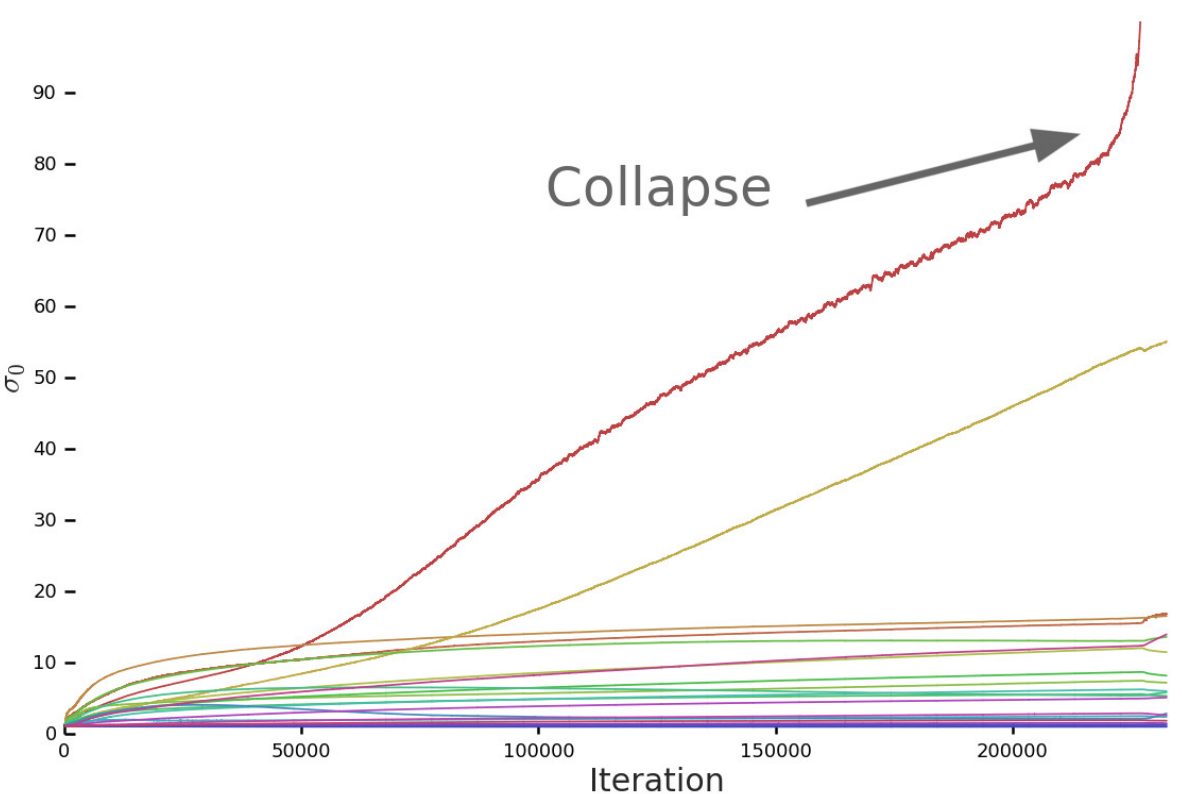
\includegraphics[width=0.7\textwidth]{images/biggan-singular-values-generator}
    \end{figure}
\end{frame}

\begin{frame}{How to track instability in Discriminator}
    \begin{itemize}
        \item\pause Singular values are much more well-behaved, they only jump at collapse and do not explored
        \item\pause Singluar values are more noisy and have spikes
        \item\pause Authors hypothesize that spikes occur because $D$ receives large gradients sometimes
        \item\pause To alleviate this they use $R_1$ regularization: it helps it decreases overall performance
        \begin{equation}
            R_{1}:=\frac{\gamma}{2} \mathbb{E}_{p_{\mathcal{D}}(x)}\left[\|\nabla D(x)\|_{F}^{2}\right]
        \end{equation}
    \end{itemize}
    
    \begin{figure}
        \centering
        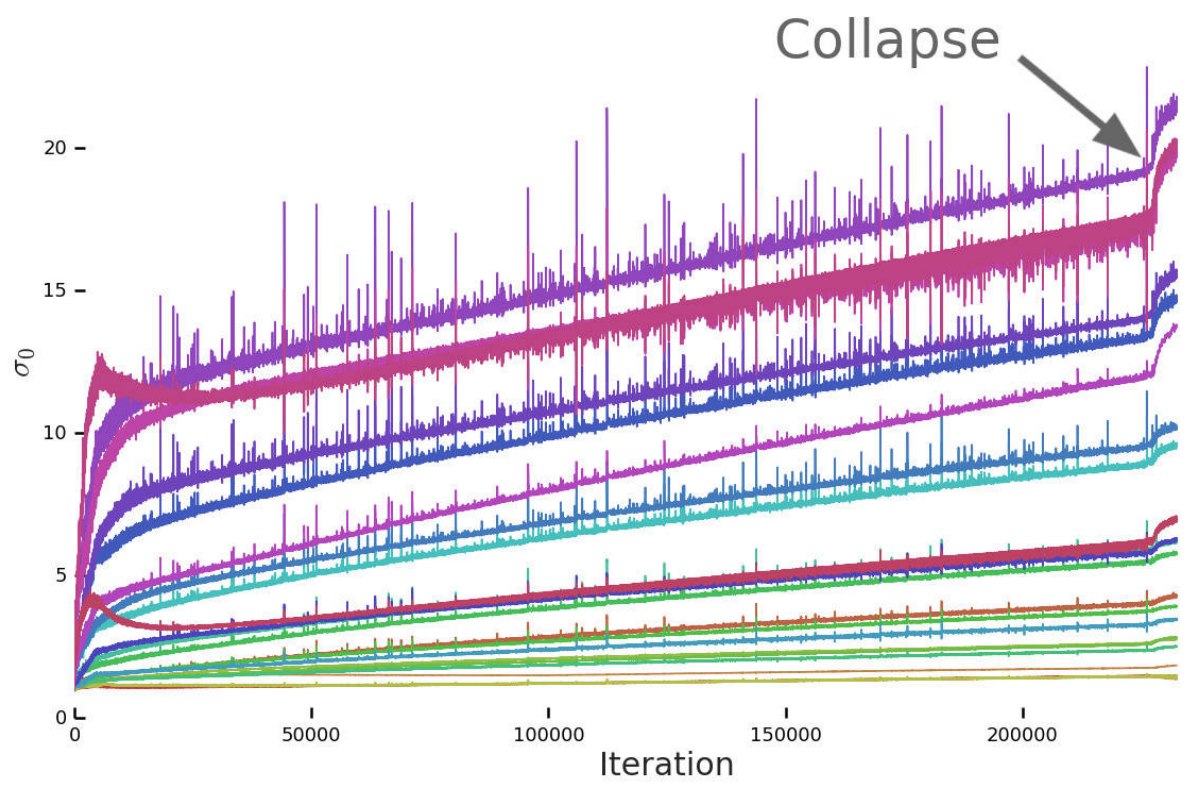
\includegraphics[width=0.5\textwidth]{images/biggan-singular-values-discriminator}
    \end{figure}
\end{frame}

\begin{frame}{Results}
    \centering
    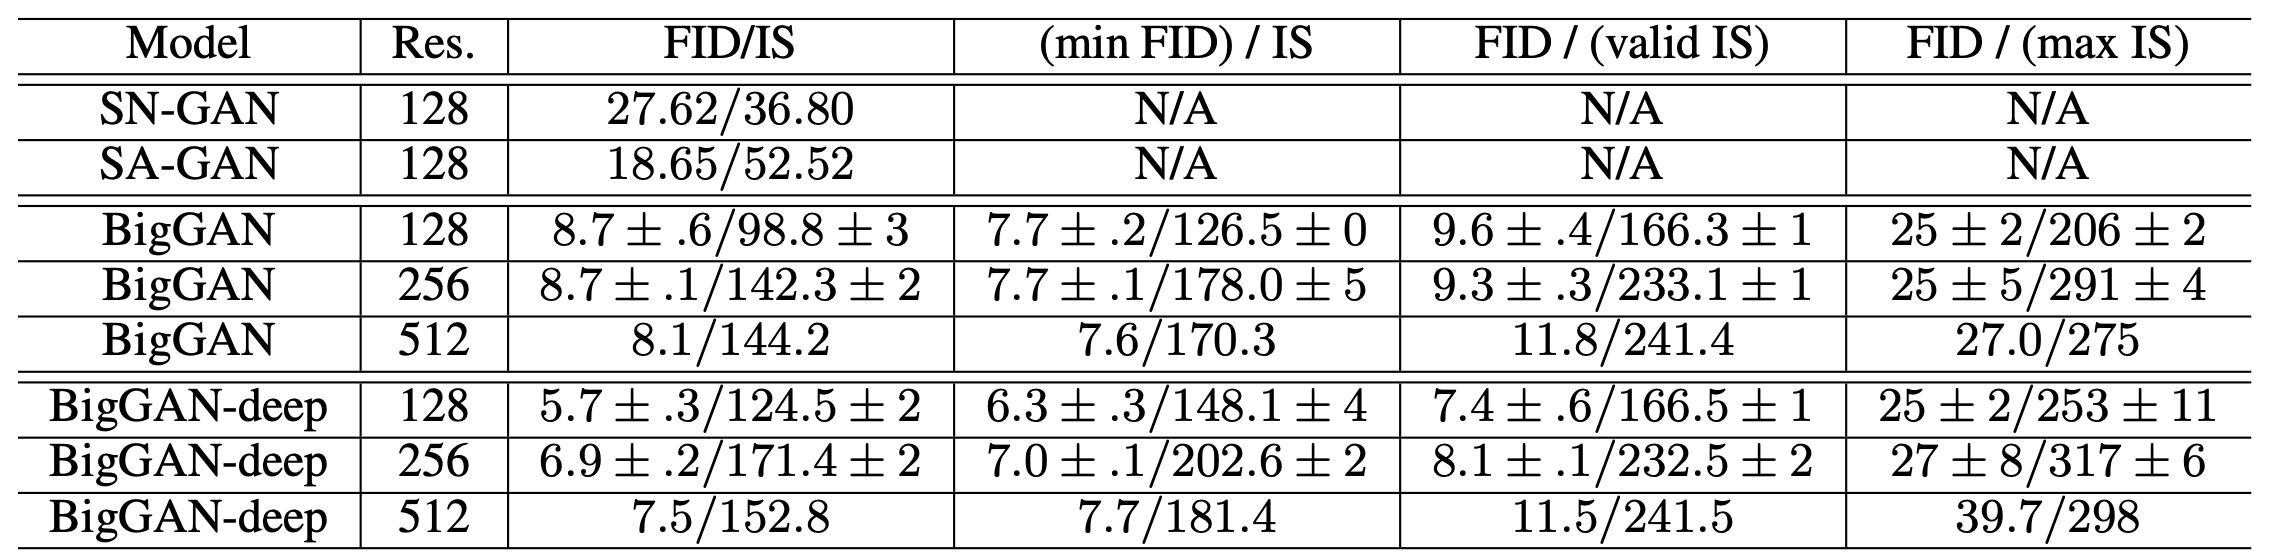
\includegraphics[width=\textwidth]{images/biggan-results}
\end{frame}

\end{document}
